\documentclass[extern,palatino]{cgBA}
\usepackage{setspace}
\usepackage{graphicx} 
%\onehalfspacing
\doublespacing

\author{Martin Groppe und Malte Kremer}
\title{Entwicklung eines AR-Rollenspiels für Android}
\zweitgutachter{...}
\externLogo{7.46cm}{logos/UniLogoNeu}
\externName{DIN: NewTechnologies}

\begin{document}

% Umschalten der Sprache (für englische Rubrikbezeichnungen etc.)
%\selectlanguage{english}


\maketitle

\newpage

\pagenumbering{roman}
\tableofcontents
\clearpage         % oder \cleardoublepage bei zweiseitigem Druck
% \listoffigures   % fuer ein eventuelles Abbildungsverzeichnis
% \clearpage
\pagenumbering{arabic}


\section{abstract}

Pokémon Go wurde in den ersten drei Monaten nach dem Release 500 Millionen mal heruntergeladen, bleibt aber als Hybrid aus Rollen- und augmented reality-Spiel eher die Ausnahme. 
\\Ziel dieser Arbeit ist es daher, vergleichbare Produkte zu analysieren und aus der Analyse einen Prototypen für ein AR-Rollenspiel zu entwickeln. Anschließend wird dieser von Testpersonen darauf geprüft, ob er Spaß macht und das Potenzial hätte, langfristig zu fesseln um allgemeine Erkenntisse über die Qualität des Prototypen zu gewinnen.
\section{abstract (english)}
Pokémon Go had enormous success, was downloaded 500 million times in the first three months. It is however a rare case of a combination of Augmented reality and role-playing game features.
\\This thesis intends to develop a role-playing game that uses Google Maps features and is fun and engaging. The implementation will then be tested and evaluated.
\newpage
\section{Motivation}
Spätestens seit dem massiven Erfolg von Pokémon Go sind Smartphones als Spieleplatform nicht mehr wegzudenken. Dennoch bleibt Pokémon Go eher eine Ausnahme insofern, dass die Verknüpfung der AR-Möglichkeiten des Smartphones selten mit klassischen Spielkonzepten kombiniert wird. Dabei hat Pokémon Go gezeigt, dass es relativ einfach ist, die reale Welt in Rollenspiele einzubauen. \\Daher haben wir es uns zum Ziel gesetzt zu erforschen, inwieweit es möglich ist, in einem relativ kurzen Zeitraum und mit geringem Budget einen Prototyp zu entwickeln, der AR-Elemente beinhalten, kurzfristig Spaß machen soll und das Potenzial haben soll langfristig zu fesseln.
\newpage
\section{Grundlagen}
Da das Spiel auf Android laufen soll, wird Interface und Basis-Programm mit java programmiert. Als Entwicklungsumgebung für den java-Code wird Google's hauseigenes Android Studio verwendet, da es gut dokumentiert und weit verbreitet ist.
\\Die Kämpfe hingegen werden mit der Unity-game-engine erstellt, sodass für die Erstellung der Grafik nur ein Bildbearbeitungsprogramm benötigt wird. Dazu wurde Adobe Photoshop verwendet.
\subsection{android}
\subsubsection{AR-Funktionen von Android}
\newpage
\subsection{Unity}
Unity ist eine 2005 von von Unity Technologies SF veröffentlichte Game engine und ist seitdem zunehmend erfolgreich. %laut wikipedia nutzen 47% der Spiele auf mobilen Geräten unity.
Sie wird von Indie-Entwicklern wie William Chyr Studios wie von Publisher-abhängigen Entwicklungsstudios wie Square Enix Montreal benutzt und ermöglicht Entwicklung ebenso für Smartphone-Betriebssysteme wie iOS, Android, Windows Phone wie auch für Mac, Windows, die Playstation 4 oder den 3DS. 
\\Insgesamt sind mit Unity über 238.000 Spiele für den mobilen Markt (Quelle: unity analytics) und etwa 34\% der Top 1000 mobilen Spiele entwickelt worden, es ist die meistbenutzte nicht-inhouse-Engine. Allein im dritten Quartal 2016 hatte Unity über fünf Milliarden downloads. Außerdem ist es benutzerfreundlich, gut dokumentiert und die große Verbreitung machen den Einstieg einfach.
\\Unity bietet die Möglichkeit in 2D sowie in 3D zu programmieren, hat Automatismen für die Erstellung von Animationen aus Spritesheets und bietet übersichtliche objektorientierte Verknüpfungen von Scripts und Game-Objekten. Unitys' Scripts müssen entweder in C\# oder in JavaScript geschrieben werden.
\newpage
\subsection{Photoshop}
Photoshop ist ein Bildbearbeitungsprogram, das 1988 von Adobe entwickelt wurde und seitdem mehrfach weiterentwickelt wurde. Mit Photoshop werden Bilder auf Pixel-basis bearbeitet. Dies ermöglicht relativ einfache Erstellung von sogenannten Sprites, Bildern die als Basismodelle für 2D-Figuren dienen.
\\
Photoshop ist in unter Game-Artists weit verbreitet und wird für die Erstellung von Storyboards, Sketches und Sprites benutzt. Animation Career Review listet es als die essenziellste Software für Künstler und Designer, Developer hat es in ihrer nicht-sortierten Top acht Liste, bloopanimation empfiehlt es ebenfalls für 2d-Animation und bezeichnet es als "großartige Wahl (great choice). 2005 war Photoshops' Marktanteil zwischen 60\% und 70\% im Bereich Bildbearbeitungssoftware für Rastergrafik (Bundeskartellamt, %http://www.bundeskartellamt.de/SharedDocs/Entscheidung/DE/Entscheidungen/Fusionskontrolle/2005/B7-162-05.pdf?\_\_blob=publicationFile\\&v=3
), 2010 hatte Photoshop über 10 Millionen Nutzer weltweit.
\\
Außerdem ist es gut dokumentiert und leicht zu lernen (eine Google-Suche nach Photoshop Tutorial lieferte rund 14.500.000 Ergebnisse). All das machte es zu einer guten Wahl für die Erstellung der Grafik.
\newpage

\section{Recherche und Konzeption}
\subsection{Rollenspiel und AR-Hybriden auf Android}
\subsubsection{Pokémon Go}
Pokémon Go ist ein freemium/free-to-play Smartphone-Spiel für iOS und Android. Es wurde von Niantic entwickelt und im Juli 2016 veröffentlicht und benutzt Google Maps sowie situational das Gyroskop und die Kamera für AR-Funtionen. 
\\Pokémon Go ist bis heute das erfolgreichste Spiel das für Smartphones erschienen ist, mit über 650 Millionen Downloads (Stand 27.02.2017) und über 500 Millionen Downloads in den ersten zwei Monaten.%http://archive.is/XCgwL
 2016 haben gleichzeitig an einem Tag 23 Millionen Nutzer gespielt.
\\
Im Folgenden wird grob die Funktionsweise von Pokémon Go erklärt. Pokémon Go benutzt GPS, um die Position der Spieler zu erfassen und auf einer Google Maps ähnlichen Karte anzuzeigen. Niantics' Server spawned Pokémon (Monster, die man fangen, trainieren und zum kämpfen benutzen kann) an mehr oder weniger zufälligen realen GPS-Positionen. Dabei berücksichtigt der Server eine Reihe von Faktoren, Pokémon vom Typ Wasser werden z.B. eher in der Nähe von Flüssen, Seen und Brunnen erschaffen, während Pokémon vom Typ Geist eine erhöhte Chance haben, bei Nacht aufzutauchen. Wenn der Spieler nah genug an ein Pokémon heran kommt, kann der Spieler das Pokémon sehen und auf es tippen, um einen Bildschirm aufzurufen, in dem sie versuchen können, es mit einem Pokéball zu fangen. Sollte es dem Spieler nicht gelingen, dass Pokémon innerhalb einer bestimmten Zeit zu fangen, entkommt es.
\\Außerdem gibt es an festgelegten Orten sogenannte Poké-Stops, an denen Spieler Items wie die vorher erwähnten Pokébälle bekommen können. Zusätzlich gibt es Arenen, an denen Spieler gegen die Pokémon von anderen Spielern kämpfen können um Items zu bekommen. Dies führt dazu, dass Spieler häufig in der realen Welt bestimmte Routen ablaufen und sich an festgelegten Orten immer wieder begegnen, was mehr oder weniger automatisch zu neuen Kontakten und Freundschaften führt. Neben den realen Kontakten mit denen man das Spiel spielen kann und den Orten, die man besucht, sorgt auch die Kamera-Anzeige in der Pokémon vor einem realen Hintergrund angezeigt werden und die Anpassung von Pokémon in Gebieten für eine Verknüpfung von realer und virtueller Welt. 
\\Das Spiel herunterladen ist kostenlos, im Shop kann man z.B. Pokébälle oder Inventar-Erweiterungen für eine Ingame-Währung kaufen, die man auch mit realem Geld kaufen kann. Nutzer die reales Geld ausgeben haben dementsprechend Vorteile, die einen schnelleren Fortschritt ermöglichen. Laut Schätzungen hat Pokémon Go 2016 etwa 950 Millionen US-Dollar Einnahmen erzeugt.%https://venturebeat.com/2017/01/17/pokemon-go-generated-revenues-of-950-million-in-2016/
\\Auch wenn Pokémon Go alle Smartphone-Spiel-Rekorde gebrochen hat, gibt es doch einige Kritik. Die Interaktionsmöglichkeiten mit anderen Spielern hielten sich stark in Grenzen, das Monetisierungs-Modell war recht unterentwickelt und es gab kein wirklich forderndes Element. Arena-Kämpfe erwiesen sich als recht repetetiv und anspruchslos und echtes Player vs Player-Gameplay, bei dem beide Seiten aktiv Einfluss auf das Kampfgeschehen nehmen können gibt es nicht. Es gibt auch keinen anderen fordernden Endgame-Inhalt, sodass viele Pokémon erst trainierten um dann festzustellen, dass sie nicht viel mit den Pokémon machen konnten. %http://archive.is/bFBtX
\newpage
\subsubsection{Parallel Kingdom}
Parallel Kingdom war ein Spiel, das Elemente aus MMORPG-, Geocache-Spielen und von Real-time browser-based MMOs wie OGame beinhaltete. Es wurde 2008 von PerBlue released und November 2016 abgeschaltet. 
\\Das Spiel mischte verschiedene typische MMO-Elemente wie Ressourcen und Items sammeln und tauschen, Dungeons erforschen, Monster bekämpfen und Fähigkeiten steigern mit einer realen Weltkarte, auf der man sich (anders als in Pokémon Go oder in unserem Spiel) auch virtuell fortbewegen konnte, der Möglichkeit Territorium zu kontrollieren und OGame Features wie Gebäuden die stetigen Ertrag bringen und PvP-Kriegen um Gebiete.\\Das Spiel war mit über 1.000.000 Spielern recht erfolgreich, wurde mehrfach für Awards nominiert und hatte mit acht Jahren eine für ein Android Spiel sehr lange Lebensdauer.  %https://www.nowgamer.com/parallel-kingdom-interview-when-mmo-meets-gps/
Die Abschaltung war laut Entwickler hauptsächlich wegen der veralteten Technik nötig. %http://www.parallelkingdom.com/community/update-hut.aspx#302
Die lange Zeit, über die das Spiel lief zeigt, dass die Konzepte gut ineinander griffen und es einiges an erzielbarem Fortschritt gab. Leider waren viele der Konzepte im Kern recht simpel, Kämpfe bestanden häufig aus nebeneinander laufen und anschließend den Gegner wiederholt anklicken (ohne ernsthafte Strategie) und wurden oft durch Items und Level entschieden. Leider kamen wir nicht dazu, die großen PvP-Funktionen zu testen, da das Spiel zum Start dieser Arbeit lange über seine Hochphase hinaus und kurz vor der Abschaltung war.
\subsection{Rollenspielen auf anderen Plattformen und Portierungen}
Rollenspiele auf dem PC-Markt setzen häufig andere Prioritäten als Smartphone Titel wie die beiden obengenannten. Viele klassischen Rollenspiele legen großen Wert auf Dialoge und ihre Geschichte. Für Skyrim wurden 83 Schauspielern für Tonaufnahmen eingestellt, fast so viele wie Entwickler, Horizon's Szenario ist eines von ursprünglich 40 verschiedenen und für die finale Story wurden etwa 20 verschiedene Entwürfe gemacht. Dragon Age: Inquisition hat über 140 Sprecher und zehn Storywriter.  %http://www.imdb.com/title/tt3763912/fullcredits?ref_=tt_cl_sm#cast %http://www.statisticbrain.com/skyrim-the-elder-scrolls-v-statistics/
%https://en.wikipedia.org/wiki/Horizon_Zero_Dawn#Development
Auch große Konsolenprojekte wie moderne Ableger der Final Fantasy-Serie legen großen Wert auf Story und Präsentation.
\\Leider fehlt uns sowohl Zeit, als auch Budget für derartige Projekte, weshalb wir uns eher an Indie-Projekten auf dem PC und "kleineren" Projekten auf den Konsolen orientieren. Das hoch gelobte the Banner Saga hat ein ausgereiftes Kampfsystem und wurde am Anfang von drei Leuten programmiert. Andere sogenannte Taktik-Rollenspiele wie Disgaea und Final Fantasy Tactics haben reduziertere Grafik und Story und konzentrieren sich eher auf vielschichtige Level-Systeme. Unser Ziel war es daher eher strategische Kämpfe und einen deutlich merkbaren Level-Fortschritt zu generieren, Dinge, die Pokémon Go fehlen.
\newpage
\subsubsection{The Banner Saga}
The Banner Saga ist ein von Stoic entwickeltes Taktik-Rollenspiel. Es wurde von drei ehemaligen BioWare-Mitarbeitern produziert, die 

\section{Implementation}
\subsection{Erstellung des Kampfes in Unity}
In Unity werden Gameobjects als Basiseinheit für die Erstellung von Spielen verwendet. Gameobjects sind Behälter denen man verschiedene Komponenten wie Sprites und Skripte hinzufügen kann. Für die Steuerung unseres rundenbasierten Kampfes generieren wir in Unity ein Gitter aus Quadraten die sich anklicken lassen und ihre Position im Gitter kennen. Damit der Kampf sich nicht immer gleich anfühlt erzeugen wir zufällig auf unseren Quadraten Steine als Hindernisse. Unsere Spielfiguren werden dann abhängig davon welche am Kampf beteiligt sind aus sogenannten Prefabs, Schablonen aus denen man ein Gameobject instanziieren kann, erzeugt und auf die Seiten des Spielfeldes gesetzt. Figuren sind nun reihum am Zug. Wenn eine Figur die dem Spieler gehört an der Reihe ist markieren wir alle Felder zu denen sie sich bewegen kann auf unserem Feld. Wird eines dieser Felder angeklickt generieren wir wie in \ref{Pfadfindung} beschrieben einen Pfad den unsere Figur dann abläuft. In unseren Prefabs sind die zugehörigen Animationen für die verschiedenen Befehle vorgemerkt. Wenn der Benutzer auf eine gegnerische Figur in Reichweite der aktiven klickt wird diese angegriffen und der Zug beendet. Alternativ kann man die aktive Figur anklicken um den Zug ohne Angriff zu beenden. Wenn die aktive Figur dem Gegner gehört übernimmt eine simple Ai die Entscheidungen die sonst der Spieler trifft. Die Ai überprüft ob eine feindliche Figur in Reichweite ist und greift diese an fals möglich. Wenn nicht bewegt sie sich auf die nächste feindliche Figur auf dem Feld zu. Falls sie nun in Reichweite ist greift sie die Figur an andernfalls beendet sie ihren Zug.
\subsection{A* Pfadfindung}\label{Pfadfindung}
Um Figuren auf unserem Spielfeld zu bewegen benötigen wir einen Suchalgorithmus um einen Pfad zu finden. Wir haben dazu den A* Algorithmus implementiert. Im Gegensatz zu uninformierten Suchalgorithmen wie Dijkstra wird in A* eine Heuristik benutzt um Zielgerichtet zu suchen. Alle Felder werden in 3 Gruppen unterteilt. Die erste Gruppe sind die noch nicht gefundenen Felder. Am Anfang sind dies alle außer dem Startfeld. Die 2. Gruppe sind die Felder zu denen mindestens ein Weg bekannt ist. Diese werden zusammen mit einem Wert f(x) in einer Liste gespeichert. Der Wert von f(x) ergibt sich aus der Summe der Kosten um den Knoten zu erreichen g(x) und den geschätzten Kosten um von dort zum Ziel zu kommen. Im Falle von unserem Spiel kostet es einen Punkt um sich orthogonal zu bewegen und 2 diagonal. Die Schätzfunktion nimmt einfach die Summe der Abstände in x und y Koordinate zwischen einem Feld und dem Zielfeld. Zusätzlich wird für jedes Feld in dieser sogenannten Open List gemerkt von welchem Feld ausgehend der momentane Weg dort ankommt. Die 3. Gruppe besteht aus den Feldern zu denen bereits ein optimaler Weg gefunden wurde. Diese Felder werden in der sogenannten Closed List ebenfalls mit dem Feld von dem der kürzeste Weg zu ihm ausgeht gespeichert.
Zu Beginn befindet sich nur das Startfeld in der Open List und die Closed List ist leer. Nun wird in jedem Schritt das Feld x mit dem geringsten f-Wert aus der Open List in die Closed List aufgenommen. Für jedes Nachbarfeld y wird nun g(y) berechnet aus g(x)+1, falls es ein orthogonaler Nachbar, und g(x)+2 , falls es ein diagonaler Nachbar ist. Zusammen mit der oben beschriebenen Heuristik wird nun f(y) = g(y)+h(y) berechnet und y wird in die Open List mit x als Vorgänger aufgenommen, falls es dort nicht schon mit einem gleichgroßen oder kleineren f-Wert vorhanden ist. Der Algorithmus endet sobald das Zielfeld in der Open List aufgenommen wird. Der Weg ergibt sich nun indem man über die gemerkten Vorgänger die Felder bis zum Start zurückverfolgt.
\subsection{Karte und Menüs auf Android}
Unser Android Code besteht aus 4 Activities. Eine Activity in Android ist eine Oberfläche in der beschrieben wird was momentan angezeigt wird und wie mit Benutzereingaben umzugehen ist. Um zwischen den Activities zu kommunizieren werden sogenannte Intents verwendet. Unsere Hauptactivity auf der der Benutzer startet besteht aus 3 Fragmenten zwischen denen man mit swipen hin und her tauschen kann. In der Mitte befindet sich unsere Karte. Auf unserer Karte wird die Position des Spielers, die über Gps abgerufen wird, und die Position von Gegnergruppen gegen die man kämpfen kann angezeigt. Wird eine Gegnergruppe angeklickt wird ein Infofenster mit näheren Informationen zu den Gegnern angezeigt über das wenn man nah genug dran ist den Kampf starten kann. Die notwendigen Daten für den Kampf werden als Json Strings serialisiert und der Unity-Player-Activity über den Intent mitgeteilt.
\begin{figure}[htb] 
	\centering
	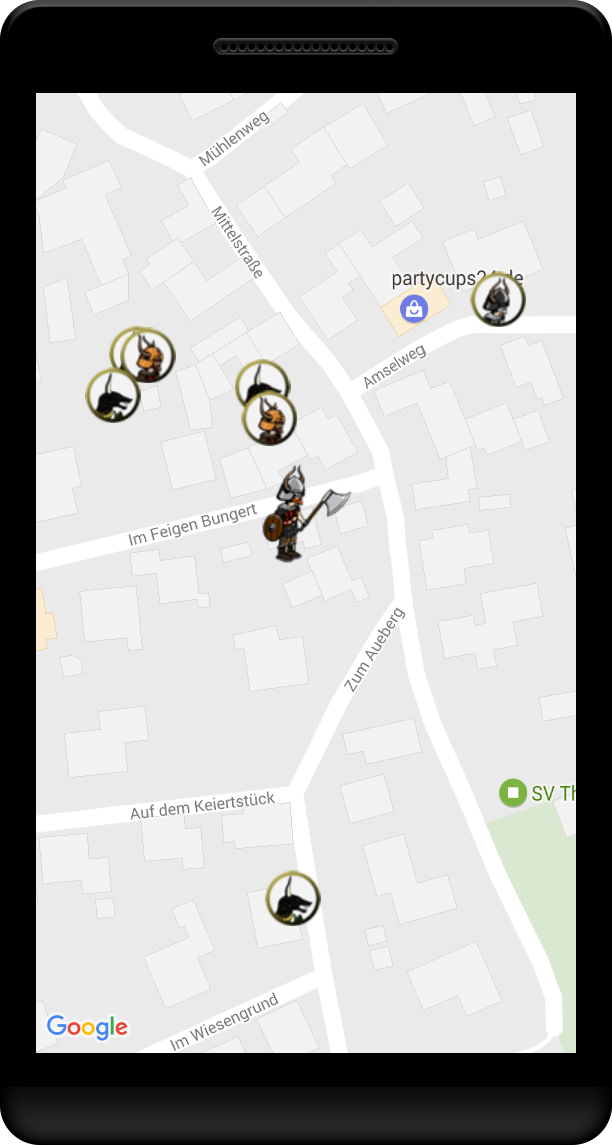
\includegraphics[width=0.4\textwidth]{map.png}
	\caption{Karte mit Spielfigur in der Mitte. Die Portraits representieren Gegnergruppen}
	\label{fig:Bild1}
\end{figure}
Im linken Fragment befindet sich unser Gruppen-Bildschirm. Auf ihm wird dem Spieler die eigene Gruppe angezeigt und er kann auswählen welche Charaktere am Kampf teilnehmen sollen. Die Charaktere in der oberen Leiste sind momentan aktiv und man kann sie indem man sie anklickt gegen einen beliebigen inaktiven Charakter austauschen.\begin{figure}[htb] 
	\centering
	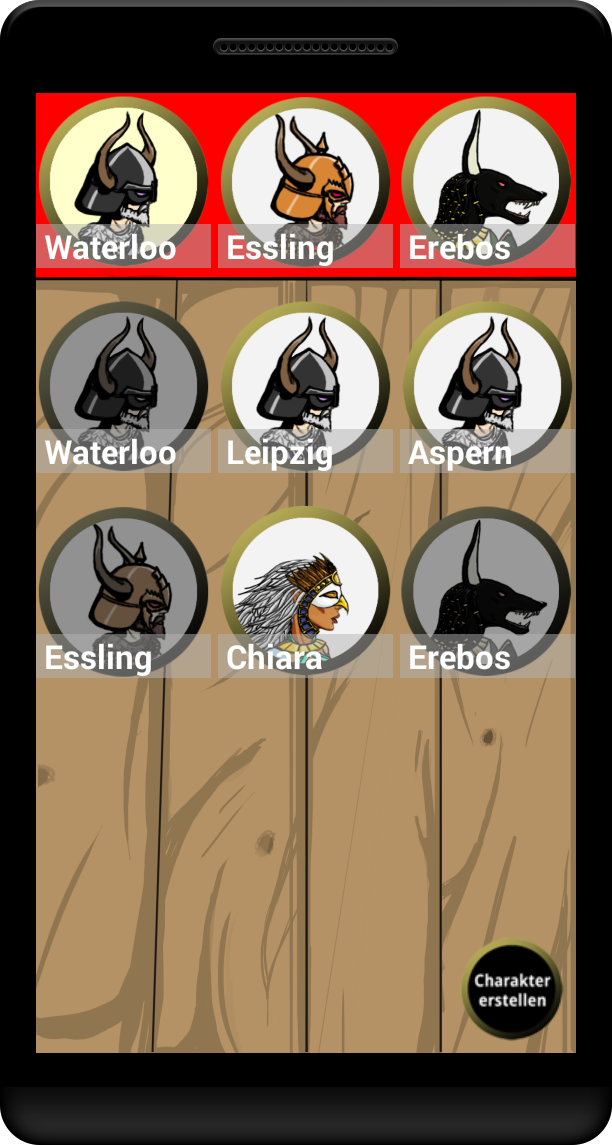
\includegraphics[width=0.4\textwidth]{charfragment.png}
	\caption{Charakter Fragment. Die aktive Party ist in der roten Leiste. Waterloo wurde angeklickt um ihn auszutauschen. Die möglichen Ziele für den Tausch sind Leipzig und Aspern}
	\label{fig:Bild2}
\end{figure} 
Wenn man auf einen Charakter im unteren Teil klickt werden die Daten des Characters in einen Intent gepackt und die StatusActivity (wir müssen unsere Bildschirme im Text besser benennen ersetze durch was du willst) wird gestartet. Über den Button unten rechts gelangt man zur Charaktererstellungs-Activity.
\newpage
Im rechten Fragment befindet sich eine Anzeige für momentane Aufgaben die der Spieler erfüllen kann um zusätzliche Belohnungen zu erhalten. Wenn der Spieler die Aufgabe erfüllt hat kann er diese über den Button abgeben und er bekommt einen zufälligen Gegenstand auf dem Level seiner Gruppe als Belohnung.
\newpage
\begin{figure}[htb] 
	\centering
	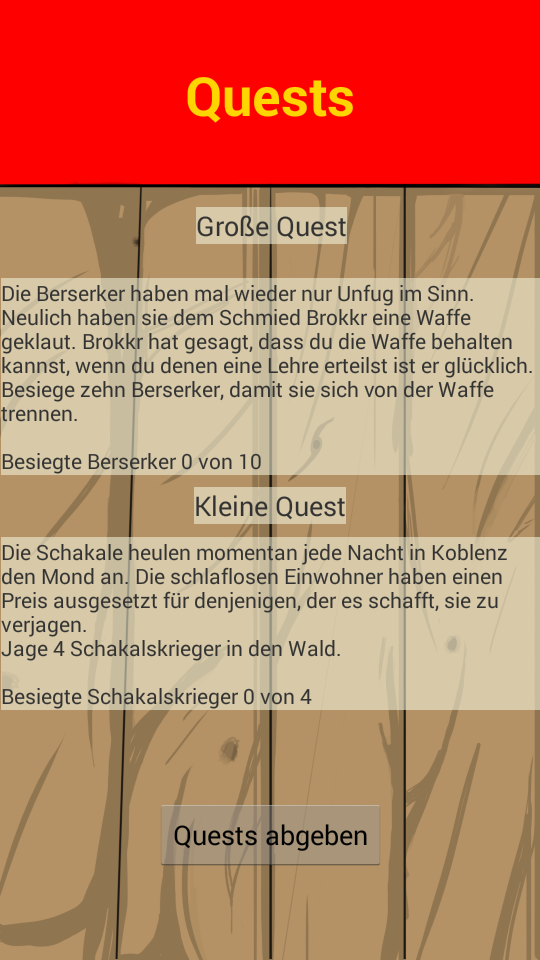
\includegraphics[width=0.4\textwidth]{questfragment.png}
	\caption{Questfragment mit momentan aktiven Aufgaben}
	\label{fig:Bild3}
\end{figure} 
Die zweite Activity ist die Unity-Player-Activity. In ihr kann der von Unity kompilierte Code abgespielt werden. Um zwischen Java und Unity-Code zu kommunizieren verwenden wir Java Native Interface, kurz JNI. JNI ist eine Programmierschnitstelle die es uns erlaubt von Unity aus Java Funktionen aufzurufen, die sich in unserer Unity-PLayer-Activity befinden. Wir benutzen JNI um die Kampfinformationen, die der Activity mitgeteilt werden, im Unity-Code abzurufen und um nachdem der Kampf fertig ist zurück zur MainActivity zu kommen.

Die dritte Activity ist die Statscreen-Activity. Hier werden die Statuswerte der Figur, die sie aufgerufen hat, angezeigt. Außerdem kann man hier der Figur gefundene Gegenstände anziehen um ihre Statuswerte zu verbessern.
\newpage
\begin{figure}[htb] 
	\centering
	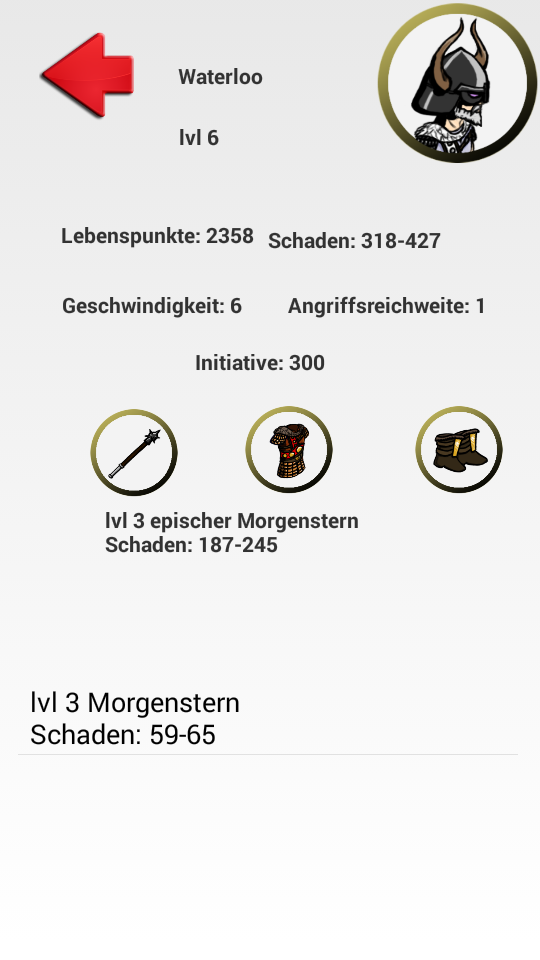
\includegraphics[width=0.4\textwidth]{statscreen.png}
	\caption{Statusbildschirm von Waterloo. Unten kann man die momentan ausgerüstete Waffe austauschen. Über die drei Symbole kann man zwischen Waffen, Rüstungen und Schuhen wechseln.}
	\label{fig:Bild4}
\end{figure} 

In der vierten Activity kann man sich eigene Charaktere erstellen. Über die vier Bilder kann man die Klasse des Charakters aussuchen und über das Textfeld einen Namen eingeben.
\newpage
\begin{figure}[htb] 
	\centering
	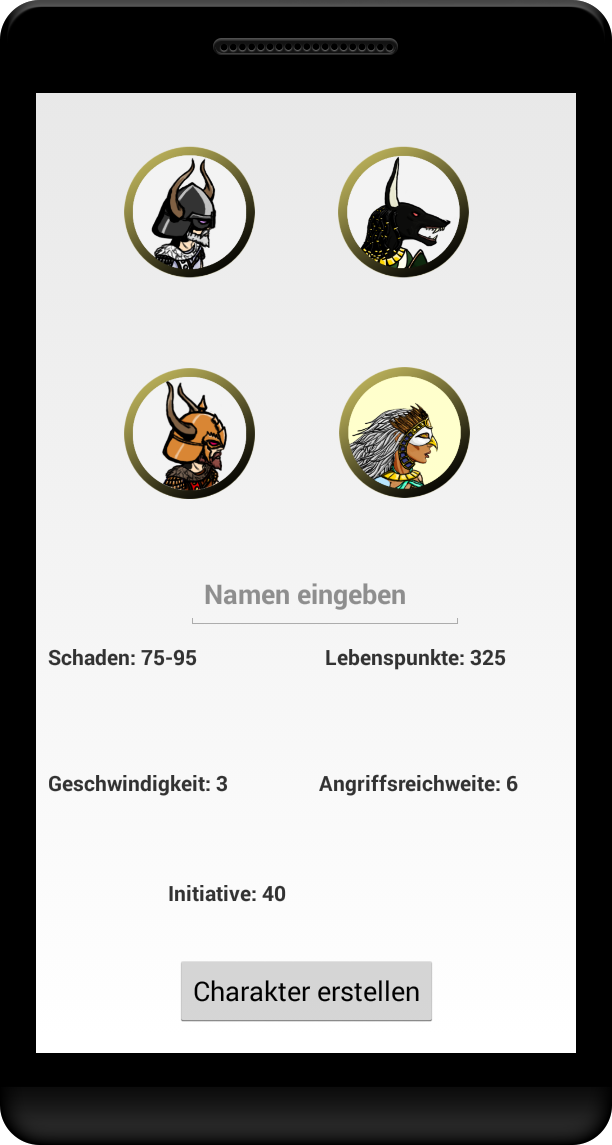
\includegraphics[width=0.4\textwidth]{createcharscreen.png}
	\caption{Hier kann man einen neuen Charakter erstellen.}
	\label{fig:Bild5}
\end{figure} 
\end{document}